
\lettrine[lines=3]{T}{}he string interpreter is one of the major components of plant generation and it is the final step in the process of procedural generation. The output of this stage of processing is dependant on what the L-system is representing, in this case it is responsible for interpreting the resulting string of modules provided by the L-system rewriter, and uses this to generate the 3D models, structures and data of the resulting plant, which is then rendered and simulated on the screen using the OpenGL framework. The generation of plant-life has three main stages, the first part consists of a turtle graphics interpreter which takes the string of modules as a set of instructions, it starts from the root of the tree and generates a skeleton made up of joints, this is similar to the techniques used in skeletal rigging in animation \cite{gregory2014game}. The joints within the tree skeleton each represents a branch segment which has some information about the properties of that segment. These segements can be used to generate the vertex, index and other data that make up the 3D models of the plant. These models can finally be passed to the final part of string interpreter which is the renderer, the renderer is reponsible for taking all the vertices, indices, textures and shaders and organising it in an optimal way that enables rendering the plant on the screen, as well as the physical simulation of the tree skeleton. The stages of string interpretation can be seen in figure \ref{l-system interpreter} below. 

\begin{figure}[htbp]
	{\centering
		\vspace{7px}
		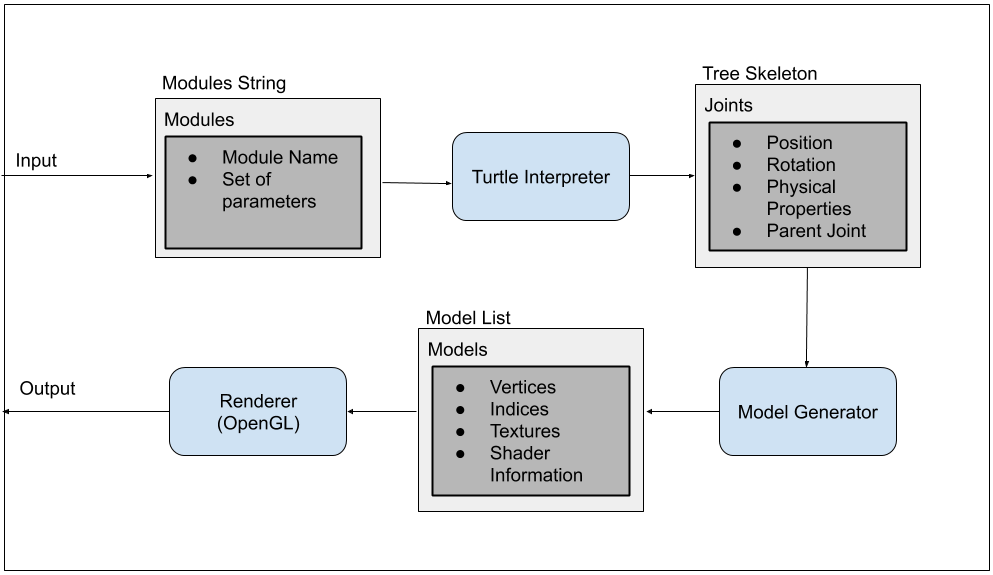
\includegraphics[scale=0.4]{Diagrams/L-systemInterpreter.png}
		\caption{Diagram of the stages of L-system interpretation and rendering} \label{l-system interpreter}
	}
\end{figure}
\FloatBarrier

\noindent
This chapter will cover each stage of the string interpreter implementation in detail, as well as well as talk about how the interpreter is able to simulate and animation the plants movements under forces such as gravity and wind in real time. 

\section{Turtle Graphics Interpreter}

The main purpose of the turtle graphics interpreter is to take the string of modules from the L-system rewriter, and interpret it as a list of turtle graphics instructions. As briefly covered in chapter \ref{l-system chapter}, each module name within the L-systems resultant string represents a particular meaning to the turtle graphics interpreter. The meaning of the module names are predefined in the string interpreter and are dependant on what the L-system is trying to represent. The L-system defined for this thesis is a parametric L-system, which allows each module to also provide a number of optional parameters. These may also carry a particular meaning for the interpreter. For instance the forward instruction or module name \say{F} can have three parameters. The value of the first parameter is the distance to move forward, this can also be seen as the length of the branch segment. The second and third parameter is the spring constant of the branch and the mass of the branch repectively. These give some information to the physics simulation in order to animate the plant. Below is a table describing the L-system module names as well as the parameter meanings for the turtle graphics interpreter.

\begin{table}[h!]
\centering
\begin{tabular}{ | c | l | l | l |}
\hline
	Instruction Name 	& Parameter 1 & Parameter 2 & Parameter 3 \\  
\hline
\hline
	F 							& Distance	& Spring Constant	& Branch Mass\\
\hline
	f 							& Distance	& Spring Constant	& Branch Mass\\
\hline
	+ 							& Angle of rotation &			&\\
\hline
	- 							& Angle	of rotation	&			&\\
\hline
	/ 							& Angle	of rotation	&			&\\
\hline
	$\backslash$ 				& Angle	of rotation	&			&\\
\hline
	$\land$ 					& Angle	of rotation	&			&\\
\hline
	\& 							& Angle	of rotation	&			&\\
\hline
	! 							& Branch width		&			&\\
\hline
\end{tabular}
\caption{Table of turtle instruction symbols and their meaning to the interpreter}
\label{instruction table 1}
\end{table}
\FloatBarrier

\noindent
Each modules instruction is carried out one by one to generate the plants skeletal structure, which is made up of joints. The joints hold information about the properties of each particular segement or object of the plant. The joints properties are the position, orientation, scale, parent joint as well as its physical characteristics. It is important to note that all of the scales and rotations must happen before the forward movement. As the rotations change the orientation of the brach and then the movement generates the joint itself. A joint is defined by the figure below:

\begin{figure}[htbp]
	{\centering
		\vspace{7px}
		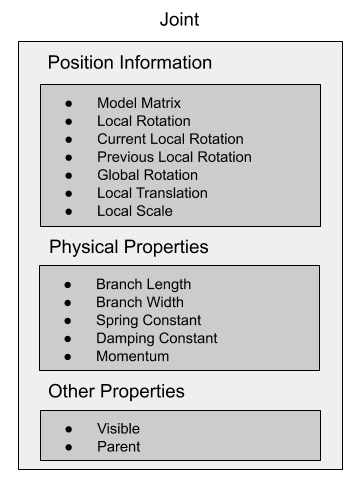
\includegraphics[scale=0.6]{Diagrams/JointDiagram.png}
		\caption{Diagram for the properties of a joint} \label{joint properties}
	}
\end{figure}
\FloatBarrier

\noindent
Figure \ref{joint properties} shows that there is in fact a large amount of information stored for the position and orientation of each joint. This is because the rotation of the joint is stored in both a local and global space. Local space refers to the rotation of the joint relative to its parent rotation, this is useful as it allows the manipulation of subsequent child joints, whilst leaving other joints local rotation unchanged. Global space, also known as world space, is the rotation of each joint relative to the world itself this is useful for understanding the current rotation of the joint relative to the world for instance calculating the torque or force calculations due to gravity. It is important to store both the current and previous rotations as they are used to calculate the rate of change for physics calculations.

The physical properties for each joint are the parts are what will affect model generation as well as physics simulations. These properties include the length, width, spring constant, damping constant as well as the current momentum of the branch. 

Take the following string of modules \say{F(1)[/(90)F(1)$\backslash$ (90)F(1)]-(90)F(1)+(90)F(1)}, the alphabet is made up of seven unique modules F, /, $\backslash$, [, ], + and -. According to the as discussed in previous chapters the \say{F} symbol represents a move forward, and \say{+}, \say{-}, \say{/}, \say{$\backslash$} symbolize different rotations, and the \say{[} and \say{]} represent save and load state respecively. The aforementioned symbols each have a single parameter except the load and save state. It is the turtle graphics interpreters job to understand what these parameters are and how to interpret them. In this case all of the \say{F} modules have the parameter value of 1, and all of the rotation modules have the parameter of 90. These are interpreted as the distance to move forward and the change in angle from the previous joint in degrees. This interpretation can be represented with the joint structure shown in figure \ref{skeleton diagram} below:

\begin{figure}[htbp]
	{\centering
		\vspace{7px}
		\setlength{\fboxrule}{1pt}
		\fbox{
			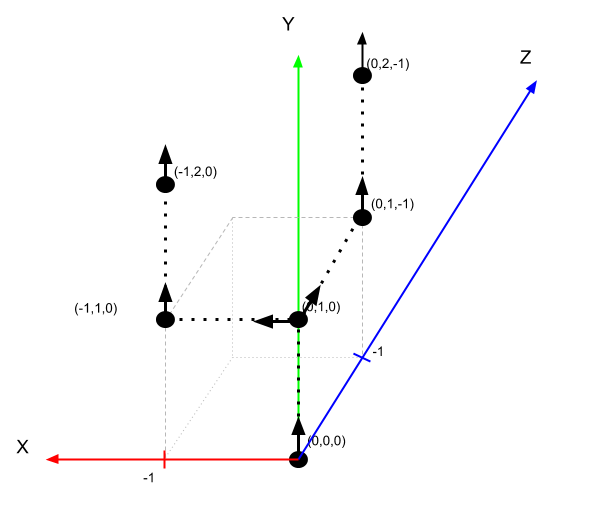
\includegraphics[scale=0.4]{Diagrams/SkeletonJoints.png}
		}
		\caption{Diagram of a simple plant skeleton with joint position and orientation.} \label{skeleton diagram}
	}
\end{figure}
\FloatBarrier

\section{Model Generator}

Modeling the branches of a plant is one of the most important parts for the overall look and feel of that plant that is being generated. The L-system described in the previous sections is able to describe the details about the plants structure, for instance the position, width, length, weight and other important information. The job of the model generator is to take this information and intelligently generate the models vertices, normals, texture coordinates and other information that can then be provided to the OpenGL renderer and finally to the GPU to be rendered on the screen.

The simplest way to generate a model for a branching structure of a plant would be to take a number of cylinders, and to rotate and stack them according to each joints position in 3D space. The up side to this approach is that every branch within the plant shares the same object model, depending on the position, rotation and scale of the branch the relavent matrix transforms can be applied. In this way we are able to represent the overall branching structure of the plant. However, there is a problem which is pointed out by Baele and Warz\'{e}e "The branches junction causes a continuity problem: to simply stack up cylinders generates a gap" \cite{baele2005real}. This can be shown in the figure below:

\FloatBarrier

\begin{figure}[htbp]
	{\centering
		\vspace{7px}
		\setlength{\fboxrule}{1pt}
		\fbox{
			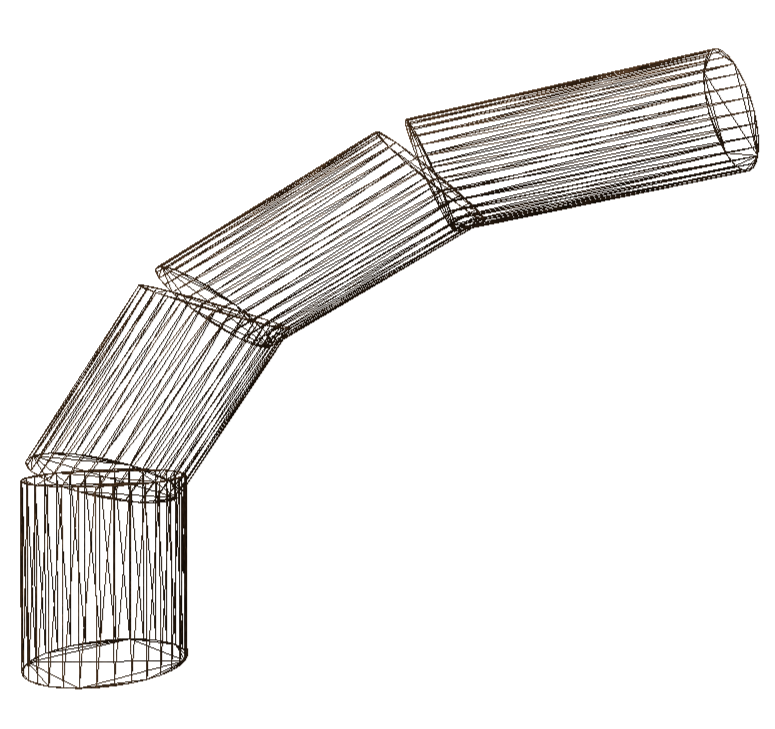
\includegraphics[scale=0.2]{Diagrams/stackedBranchesMesh.png}
		}
		\caption{Example of the continuity problem faced with stacked branching with a 25$^{\circ}$ bend per joint.}
	}
\end{figure}

\FloatBarrier

\noindent
This simple method of stacking cylinders gives a reasonable looking tree structure and it is usually good enough when the angles of branches are not more than 25$^{\circ}$ and the size of the branches do not change. However for a much more convincing tree structure there will need to be a better solution. The logical next step would be to actively link the branch segments together. This requires a number of things to take place, first of all the vertices from the previous branch top must be linked with the new top of the branch. These are the circles of vertices at either end of each branch segment. These circles will have to rotate depending on the bending direction of the branch. This means that the final model will not be made up of a large number of the same model but rather a single model with many linked branches. An example of this can be seen below:

\begin{figure}[htbp]
	{\centering
		\vspace{7px}
		\setlength{\fboxrule}{1pt}
		\fbox{
			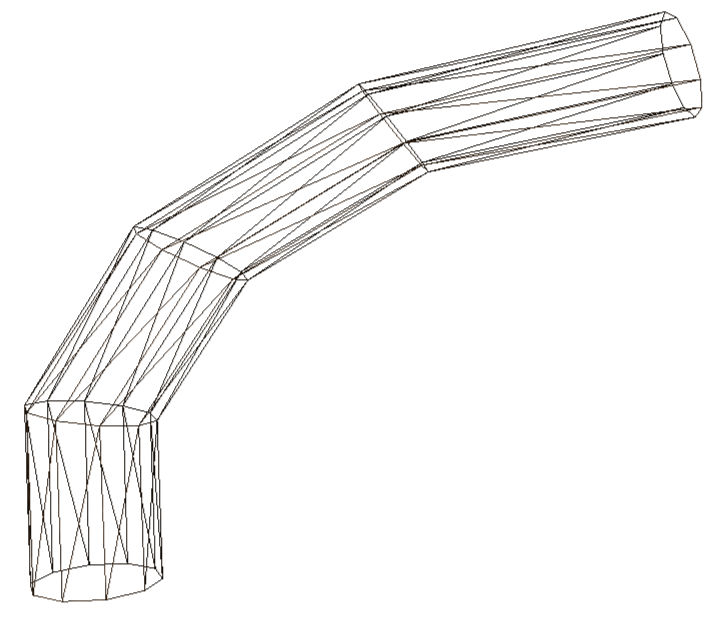
\includegraphics[scale=0.2]{Diagrams/linkedBranchesMesh.png}
		}
		\caption{Example of linked branching with a 25$^{\circ}$ bend per joint.}
	}
\end{figure}
\FloatBarrier

\noindent
This method of branch generation gives a very similar result at first glance to that of stacking cylinders. Although it does have a number of advantages, firstly it completely avoids the branch gap problem that happens with angle changes as well as branch size changes. It also means that the resolution is dynamic, meaning the number of vertices that make up a cylinder can be dynamically changed. This means that a very high resolution tree can be rendered which may look very smooth but will take a lot more computational resources, or a very low resolution tree can be rendered with more jagged edges but will require a lot less computational resources. This can be seen in figure \ref{stackedvslinked} below, where similar a looking branch can be acheived using less than half the number of vertices, with joined branches instead of stacked branches.

\begin{figure}[htbp]
	{\centering
		\vspace{7px}
		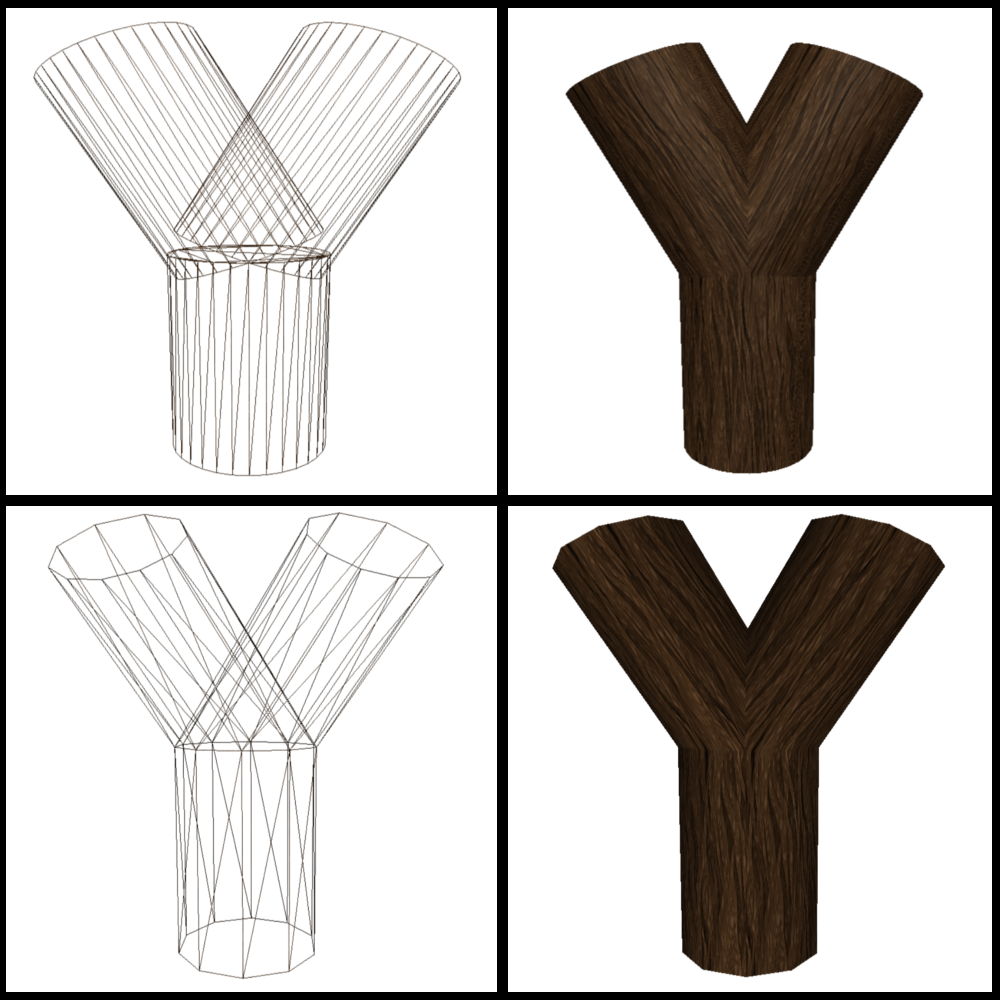
\includegraphics[scale=0.2]{Diagrams/StackedVsLinked.png}\label{stackedvslinked}
		\caption{Stacked Vs Linked.}
	}
\end{figure}
\FloatBarrier



\section{Renderer}

\noindent
The renderer is the final stage in the procedural generation pipeline. It takes all of the 3D models generated by the model generator, such as leaves, branches and flowers and renders them on the screen.  For this thesis, the \acrlong{opengl} (\acrshort{opengl}) application programming interface is use used to efficiently render the models on the screen using the \acrlong{gpu} (\acrshort{gpu}). 

The \acrshort{gpu} is a specially designed piece of harware for processing computer graphics and image processing, it has hundereds or even thousands of individual compute cores which can be used in parallel. Due to the highly parallel nature of the \acrshort{gpu}, the \acrshort{opengl} framework helps to abstract the hardware and create an interface to interact with the \acrshort{gpu} in a simpler way. There are a number of other types of graphics \acrshort{api} such as Vulkan, Metal or DirectX. These \acrshort{api}s all provide a way of interacting with the hardware behind the scenes, However, they each have a different approach. Therefore, this section will not be be going into great detail about about the specifics of \acrshort{opengl} but rather the general concepts required for rendering the plant model on the screen. The main parts of the rendering stage has to do with how model data is stored into buffer objects, secondly how textures are stored and then mapped to a certain object and thirdly how lighting can be calculated for a procedurally generated object.

\subsection{Models and Buffer Objects}

The model generator produces all of the information neccessary for the renderer to produce the result on the screen. In general the model data will consist of vertex data, texture co-ordinates and vertex normals. The vertex data is simply position of a point within a model, three vertices make up a face and the faces are what are ultimately rendered on the screen. The texture co-ordinates are the locations on a texture image which maps directly to the model vertices. Finally the vertex normals simply known as normals are the average normal vector. A normal vector being the vector that is purpendicular to the surface at a given point, and can be used for Phong shading or other types of lighting techniques.  

One of the most important parts of the rendering process is buffering the model data onto the \acrshort{gpu}. The \acrlong{vbo} (\acrshort{vbo}) is a data structure within the \acrshort{opengl} library which can be used to store this data on the \acrshort{gpu}. Generally, the data is stored as a single buffer or array with the first 3 values being a vertex position, the second two being a texture co-ordinate and the last three being a vertex normal. 

\begin{figure}[htbp]
	{\centering
		\vspace{7px}
		\setlength{\fboxrule}{1pt}
		\fbox{
			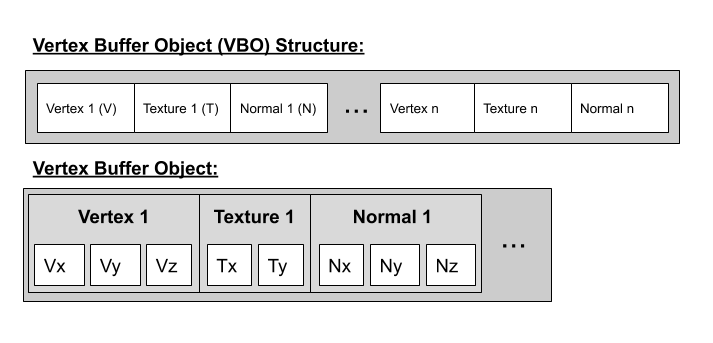
\includegraphics[scale=0.5]{Diagrams/VertexObjects.png}
		}
		\caption{Diagram showing the structure of a vertex buffer object.}
	}
\end{figure}
\FloatBarrier

Buffer objects can be created not only for the plant as a whole but potentially for different parts of the plant. For instance, the leaves on the tree are all quite similar. There is no need to have thousands of copies of a leafs vertices and textures. This would be highly wasteful and unnecessary. Simply, there could be one copy of the vertex data and texture data and instanced renderering can be used to render many copies of this object in at different places in one scene. 

\section{Shaders}

\section{Summary}








